\subsection{Grundlegender Ablauf des Programmes}
\label{subsec:grundlegender-ablauf-des-programmes}

Im folgenden Unterkapitel wird der geplante Ablauf der Applikation grundlegend beschrieben.
Hierzu wird ein Ablaufdiagramm zur visuellen Unterstützung verwendet.

Abbildung \ref{fig: Grundlegedes Ablaufdiagramm der Nutzung der Web-Applikation} zeigt den geplanten Ablauf der Datenverarbeitung innerhalb der entwickelten Web-Applikation.
Der Prozess beginnt mit dem Einlesen der XML-Dateien, die die Prüf- und Messdaten enthalten.
Anschließend erfolgt eine Validierung der Datenstruktur und des Formats, um sicherzustellen, dass die XML-Dateien den definierten Spezifikationen entsprechen.
Bei fehlerhaften oder unvollständigen Dateien wird der Prozess abgebrochen.
Sind die Daten gültig, werden sie mit den vorhandenen Datenbankeinträgen abgeglichen.
Abhängig vom Ergebnis werden entweder fehlende Datensätze ergänzt oder neue Einträge vollständig eingefügt.
Dadurch wird sichergestellt, dass die Datenbank stets konsistente und aktuelle Informationen enthält.

Nach dem erfolgreichen Datenimport erfolgt die Auswahl eines Datensatzes, dessen Inhalte grafisch dargestellt werden.
Optional kann der erzeugte Graph als PNG-Datei gespeichert werden.



\begin{figure}[H]
    \centering
    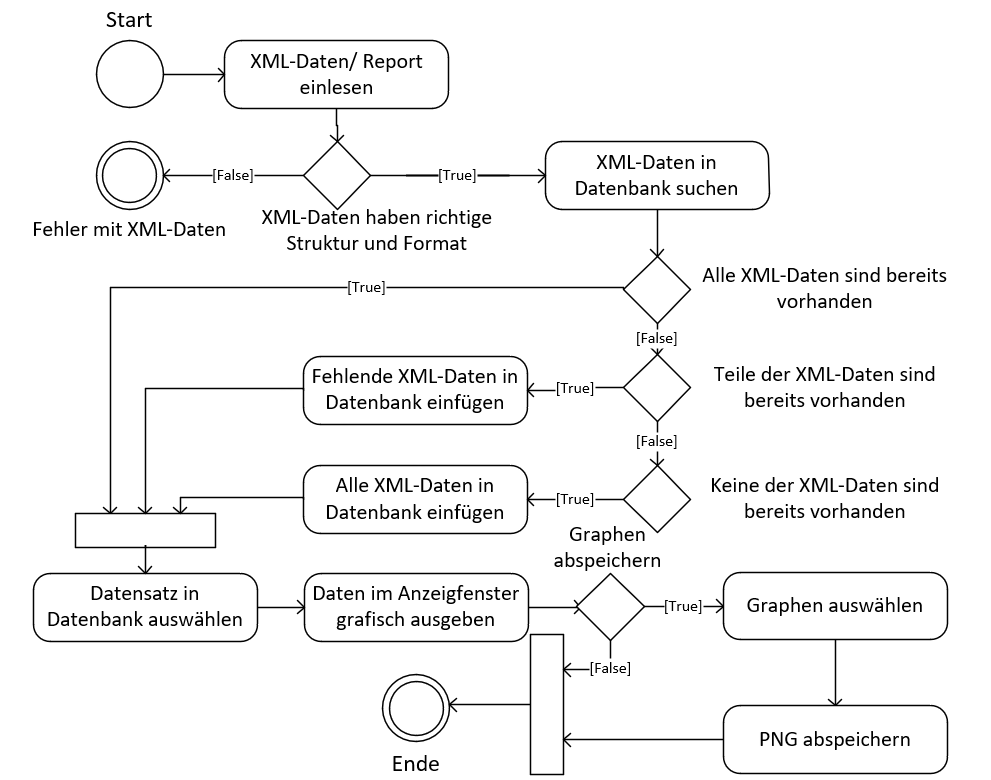
\includegraphics[width=0.95\textwidth]{Grafiken/Ablaufdiagramm}
    \caption{Grundlegedes Ablaufdiagramm der Nutzung der Web-Applikation}
    \label{fig: Grundlegedes Ablaufdiagramm der Nutzung der Web-Applikation}
    {Quelle: Eigene Darstellung mit Microsoft Visio}
\end{figure}